% Provenance (never printed): see sources/outline_sources.md (Year 2: field and laboratory methods ---
% igneous and metamorphic petrography, chemical analysis by XRF, ICP-MS and microprobe, isotope mass
% spectrometry, a mapping campaign). Modelled on Book 3 ch. 6.
% Textures: BGS RR 99-02 (Robertson 1999), Open University Virtual Microscope, Carleton BH250,
% UCSB Geology 102C (Hacker); QAPF: BGS RR 99-06 (Gillespie and Styles 1999); instruments: SERC
% Geochemical Instrumentation and Analysis sheets (EPMA, WDS, XRF, TIMS, MC-ICPMS); XRF procedure
% and reference-material results: USGS OFR 02-223 and its chapter T (Taggart and Siems 2002); Sr
% isotopes: CIAAW; spike and mass bias: Cheong, Jeong and Kwon (2014). Ledger rows in
% sources/ledger/book4.md; curves and stations from figdata/bachelor-2/labmethods.py, numbers from
% the Book 4 second-writer scratch calculator calc/ch31.py. Observation only: the professional work
% is described in the third person.
\chapter{क्षेत्र और प्रयोगशाला विधियाँ II}\label{ch:b2:field-lab-methods-2}

इस पुस्तक के शैलिकी अध्यायों की हर संख्या का आरंभ एक थैले में रखी चट्टान, सूक्ष्मदर्शी के नीचे एक पतली काट
और किसी उपकरण में रखे चूर्ण से हुआ। किसी प्रावस्था आरेख पर अंकित खनिज-संघटन, वह सिलिका-मात्रा जो
किसी लावा को नाम देती है, वह स्ट्रॉन्शियम समस्थानिक अनुपात जो प्रावार के किसी स्रोत का अनुरेखण करता है:
हर एक संक्रियाओं की ऐसी शृंखला से निकला जो किसी अनावरण पर आरंभ हुई, और हर एक में हर कड़ी की
त्रुटियाँ समाई हैं। यह अध्याय वार्डन पहाड़ियों के आधार-शैल की चट्टानों के लिए उस शृंखला का अनुसरण करता है:
पतली काट में बनावटें पढ़ना, खनिजों की गिनती, पूरी चट्टान का विश्लेषण, फिर एकल खनिजों का, फिर समस्थानिकों का,
और हर चरण पर यह पूछना कि संख्या कितनी अच्छी है।

\begin{recall}
\textbf{पुस्तक 3 (स्नातक वर्ष 1) से}: क्षेत्र-स्टेशन, क्षेत्र नोटबुक, अभिमुखित नमूना, पतली काट,
ध्रुवण सूक्ष्मदर्शी, समतल-ध्रुवित प्रकाश, आड़े ध्रुवक; शैल-निर्माणकारी खनिजों की प्रकाशिक
पहचान; ऑक्साइड विश्लेषण से ऑक्सीजनों की निश्चित संख्या पर खनिज-सूत्र का पुनःपरिकलन,
और आवेश-संतुलन से फ़ेरिक लोहे का; पर्णन और शिस्टता; समकालरेखा, आरंभिक अनुपात और
न्यूनतम-वर्ग रेखा। \textbf{रसायन की पुस्तकों से}: द्रव्यमान स्पेक्ट्रममिति, प्रेरणिक युग्मित प्लाज़्मा;
अंशांकन वक्र, संसूचन सीमा, मात्रांकन सीमा, परिशुद्धता, यथार्थता, पूर्वाग्रह,
पुनरावर्तनीयता, माध्य का मानक विचलन। \textbf{भौतिकी की पुस्तकों से}: अभिलाक्षणिक एक्स-किरणें
और मोज़ली का नियम; ब्रैग का नियम; पृष्ठ-तनाव; अनिश्चितताओं का संचरण।
\textbf{गणित की पुस्तकों से}: द्विपद बंटन, उसका माध्य और प्रसरण।
\textbf{\cref{ch:b2:magmatic-series} से}: \omterm{def:b2:magmatic-series:qapf}{मोडल संघटन}, \omterm{def:b2:magmatic-series:qapf}{QAPF आरेख}।
\textbf{\cref{ch:b2:isotope-geochemistry} से}: \omterm{def:b2:isotope-geochemistry:tracer}{रेडियोजनित समस्थानिक अनुरेखक}, \omterm{def:b2:isotope-geochemistry:standards}{समस्थानिक संदर्भ मानक}।
\end{recall}

\section{शैलवर्णन: इतिहास के रूप में बनावटें}\label{sec:b2:field-lab-methods-2:petrography}

पुस्तक 3 (स्नातक वर्ष 1) ने खनिजों को पहचानने के लिए ध्रुवण सूक्ष्मदर्शी का उपयोग किया। कोई शैलवर्णनकर्ता यह भी पढ़ता है
कि कण कैसे व्यवस्थित हैं, क्योंकि यह व्यवस्था उस क्रम को दर्ज करती है जिसमें वे बढ़े। दो
बनावटें गलित से क्रिस्टलन की और ठोस अवस्था में पुनःक्रिस्टलन की सबसे आम
साक्षी हैं।

\begin{definition}[ओफ़िटिक बनावट, ग्रैनोब्लास्टिक बनावट]\label{def:b2:field-lab-methods-2:textures}
किसी आग्नेय चट्टान की \emph{ओफ़िटिक बनावट}\index{ओफ़िटिक बनावट} तब होती है जब पाइरॉक्सीन के बड़े क्रिस्टल
प्लैजियोक्लेज़ की छोटी, यादृच्छिक दिशाओं वाली पट्टिकाओं को घेर लेते हैं; यह बनावट डोलेराइट, गैब्रो
और बेसाल्ट की विशिष्ट है। किसी कायांतरित चट्टान की \emph{ग्रैनोब्लास्टिक बनावट}\index{ग्रैनोब्लास्टिक बनावट} तब होती है जब
वह लगभग समविमीय, लगभग समान आकार के क्रिस्टलों का समुच्चय होती है, अनेक स्थितियों में अनाकृतिक,
जिनकी सीधी सीमाएँ तीन-तीन करके \ang{120} के निकट कोणों पर मिलती हैं।
\end{definition}
% ledger: carletonB:ophitic, ouVM:textures, bgsM:textures

किसी ओफ़िटिक चट्टान में घिरी हुई पट्टिकाएँ पूरी और स्वआकृतिक होती हैं, और पाइरॉक्सीन उनके बीच का स्थान
भरता है: प्लैजियोक्लेज़ पहले बढ़ा, पाइरॉक्सीन उसके चारों ओर। \omterm{def:b2:field-lab-methods-2:textures}{ग्रैनोब्लास्टिक बनावट} के \ang{120} कोण
उन कणों के हैं जिन्हें अपनी सीमाएँ समायोजित करने का समय मिला है; शैलवर्णन की शिक्षण-सामग्री ऐसी त्रिसंधियों
को रासायनिक और बनावटी साम्य का चिह्न मानती है। यह कोण बलों के संतुलन से निकलता है: कण-सीमाएँ अपनी
उभयनिष्ठ रेखा को साबुन की झिल्लियों की तरह खींचती हैं (पृष्ठ-तनाव, भौतिकी की पुस्तकों से)।
% ledger: ouVM:equilibrium

\begin{proposition}[किसी त्रिसंधि पर कोण]\label{prop:b2:field-lab-methods-2:triple}
मान लीजिए तीन कण-सीमाएँ एक रेखा के अनुदिश मिलती हैं, जिनके तनाव (प्रति एकांक क्षेत्रफल ऊर्जाएँ) $\gamma_1$,
$\gamma_2$, $\gamma_3$ हैं, और मान लीजिए $\theta_i$ सीमा $i$ के अतिरिक्त अन्य दो सीमाओं के बीच का
कोण है। साम्य पर,
\begin{equation}
\frac{\gamma_1}{\sin\theta_1} = \frac{\gamma_2}{\sin\theta_2} = \frac{\gamma_3}{\sin\theta_3},
\label{eq:b2:field-lab-methods-2:lami}
\end{equation}
और तीन समान तनाव \ang{120} के तीन कोणों पर मिलते हैं।
\end{proposition}

\begin{proof}
संधि के लंबवत किसी तल में, हर सीमा संधि को अपने ही अनुरेख के अनुदिश प्रति एकांक लंबाई $\gamma_i$ बल से
खींचती है। साम्य पर तीनों बलों का योग शून्य होता है, इसलिए सिरे-से-पूँछ रखने पर वे एक त्रिभुज
बंद करते हैं। त्रिभुज में भुजा $\gamma_i$ के सम्मुख कोण
$\pi - \theta_i$ है, जिसकी ज्या $\sin\theta_i$ है, और त्रिभुज में ज्या-नियम
\eqref{eq:b2:field-lab-methods-2:lami} देता है। यदि तीनों तनाव बराबर हों, तो त्रिभुज
समबाहु है, और हर बाह्य कोण $\theta_i$ का मान $\pi - \pi/3 = 2\pi/3$, अर्थात् \ang{120}, है।
\end{proof}

\begin{omfigure}
\centering
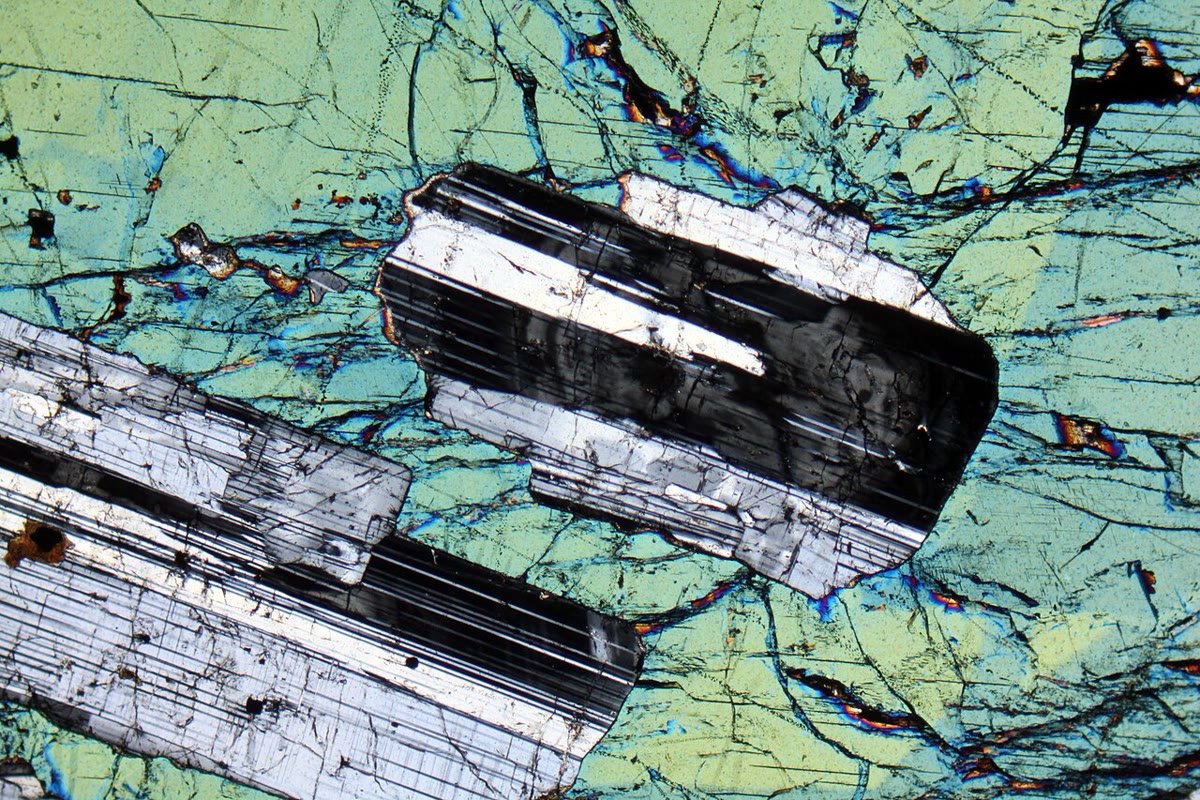
\includegraphics[height=4.6cm]{images/book4/b2-31-ophitic.jpg}\quad
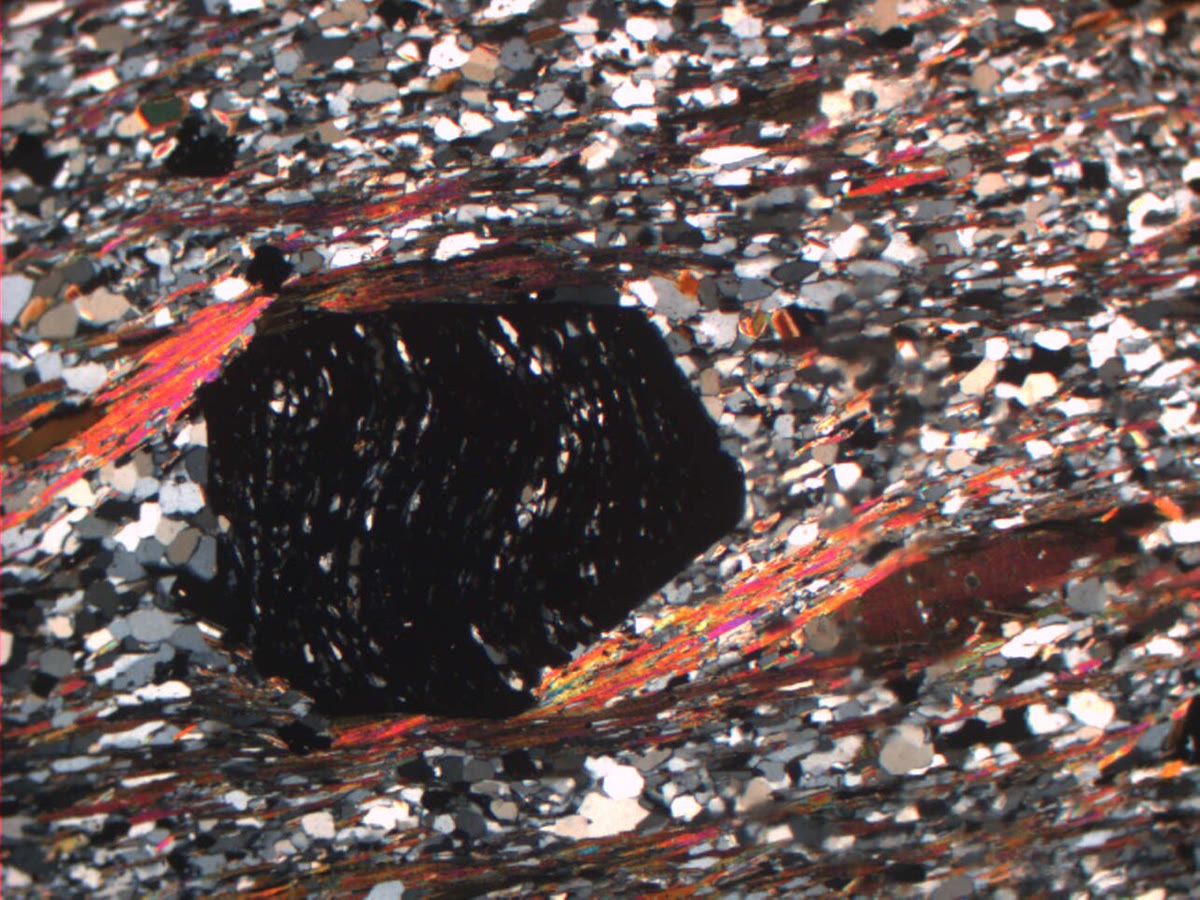
\includegraphics[height=4.6cm]{images/book4/b2-31-garnet-porphyroblast.jpg}
\par\smallskip{\small आड़े ध्रुवकों के बीच दो बनावटें। बाएँ: ऑगाइट का एक अकेला क्रिस्टल (नीला
और हरा) अपने यमलन से धारीदार प्लैजियोक्लेज़ की पट्टिकाओं को घेरे हुए है, जो \omterm{def:b2:field-lab-methods-2:textures}{ओफ़िटिक
बनावट} की व्यवस्था है; दृश्य-क्षेत्र \qty{7}{mm}। फ़ोटो: Strekeisen, CC BY-SA 4.0 (Wikimedia Commons)।
दाएँ: एक गार्नेट--अभ्रक शिस्ट। गार्नेट, जो समदैशिक होने के कारण काला है, एक बड़ा क्रिस्टल है जो
ठोस अवस्था में बढ़ा; क्वार्ट्ज़ के अंतर्वेश पंक्तियों में उसे पार करते हैं, और मस्कोवाइट
(चमकीले रंग), बायोटाइट (भूरा) और क्वार्ट्ज़ (धूसर) का पर्णन उसके चारों ओर मुड़ता है। फ़ोटो: Jackdann88,
CC BY 3.0 (Wikimedia Commons)।}
\end{omfigure}
% ledger: photo:b2-31-ophitic, photo:b2-31-garnet

कायांतरी खनिज सभी एक ही गति से नहीं बढ़ते। कुछ प्रजातियाँ बाकियों पर चढ़कर बहुत बड़े क्रिस्टल बना लेती हैं,
जो बढ़ते हुए अपने आसपास के छोटे कणों को निगल लेते हैं।

\begin{definition}[पॉर्फ़िरोब्लास्ट, पॉइकिलोब्लास्ट, अंतर्वेश-पथ, कोरोना]\label{def:b2:field-lab-methods-2:porphyroblast}
\emph{पॉर्फ़िरोब्लास्ट}\index{पॉर्फ़िरोब्लास्ट} एक बड़ा क्रिस्टल है जो \omterm{def:b2:metamorphic-facies:metamorphism}{कायांतरण} के दौरान किसी
अधिक सूक्ष्म-कणिक आधारद्रव्य के भीतर बढ़ा; गार्नेट, स्टॉरोलाइट, कॉर्डिएराइट और क्लोरिटॉइड इन्हें बनाते हैं,
जिनका आर-पार माप मिलीमीटरों से कई सेंटीमीटरों तक होता है। \emph{पॉइकिलोब्लास्ट}\index{पॉइकिलोब्लास्ट}
ऐसा पॉर्फ़िरोब्लास्ट है जिसमें अन्य खनिजों के अनेक अंतर्वेश हों। \emph{अंतर्वेश-पथ}\index{अंतर्वेश-पथ}
किसी पॉर्फ़िरोब्लास्ट के भीतर संरेखित अंतर्वेशों की एक पंक्ति है, जो
आधारद्रव्य के उस विन्यास को सुरक्षित रखती है जो उस समय था जब क्रिस्टल उस पर चढ़कर बढ़ा। \emph{कोरोना}\index{कोरोना (अभिक्रिया-बनावट)}
एक या अधिक नए खनिजों का वह घेरा है जो टूट रहे किसी खनिज को पूरी तरह
घेरता है, क्योंकि वह अपने पड़ोसियों के साथ स्थायी नहीं रह गया था: एक अभिक्रिया-बनावट,
जो अभिक्रिया के पूरा होने से पहले जम गई।
\end{definition}
% ledger: bgsM:textures, ouVM:textures

\omterm{def:b2:field-lab-methods-2:porphyroblast}{अंतर्वेश-पथ} ($S_i$, आंतरिक विन्यास) की तुलना क्रिस्टल के बाहर के पर्णन ($S_e$, बाह्य विन्यास) से करके
किसी \omterm{def:b2:field-lab-methods-2:porphyroblast}{पॉर्फ़िरोब्लास्ट} की वृद्धि का काल उस विरूपण के सापेक्ष निर्धारित होता है जिसने पर्णन बनाया। नीचे की
कसौटियाँ, जो चित्र में दिखाई गई हैं, मानक शिक्षण-टिप्पणियों की हैं।
% ledger: ucsbH:inclusion-trails

\begin{method}[अंतर्वेश-पथों से किसी पॉर्फ़िरोब्लास्ट का काल-निर्धारण]\label{met:b2:field-lab-methods-2:timing}
पर्णन के लंबवत कटी एक काट खोजिए, फिर $S_i$ और $S_e$ की तुलना कीजिए।
\begin{enumerate}
  \item \textbf{यादृच्छिक अंतर्वेश}, $S_e$ क्रिस्टल के चारों ओर विक्षेपित: वह पर्णन बनने से
        पहले बढ़ा (\emph{पूर्व-विवर्तनिक})।
  \item \textbf{किनारे पर कटा हुआ सीधा $S_i$}, विक्षेपित $S_e$ से असतत: वह
        किसी पुराने पर्णन पर, दो विरूपणों के बीच बढ़ा (\emph{अंतर-विवर्तनिक})।
  \item \textbf{वक्र $S_i$}, $S_e$ से सतत: वह पर्णन बनते समय बढ़ा, बढ़ते हुए घूमता
        रहा या ढकता गया (\emph{सह-विवर्तनिक}; हिमगोल गार्नेट की सर्पिल)।
  \item \textbf{सीधा $S_i$, अविक्षेपित $S_e$ से सतत}: वह पर्णन के बाद
        बढ़ा (\emph{उत्तर-विवर्तनिक})।
\end{enumerate}
\end{method}

\begin{omfigure}
\centering
\begin{tikzpicture}[x=1cm, y=1cm, font=\scriptsize]
% schematic after the criteria of ledger ucsbH:inclusion-trails
% panel 1: pre-tectonic
\begin{scope}[shift={(0,0)}]
\draw[omExo, line width=0.5pt] (-1.5,0.95) .. controls (-0.6,0.95) and (-0.5,0.85) .. (0,0.85) .. controls (0.5,0.85) and (0.6,0.95) .. (1.5,0.95);
\draw[omExo, line width=0.5pt] (-1.5,-0.95) .. controls (-0.6,-0.95) and (-0.5,-0.85) .. (0,-0.85) .. controls (0.5,-0.85) and (0.6,-0.95) .. (1.5,-0.95);
\draw[omExo, line width=0.5pt] (-1.5,0.45) .. controls (-0.9,0.45) and (-0.85,0.78) .. (0,0.78) .. controls (0.85,0.78) and (0.9,0.45) .. (1.5,0.45);
\draw[omExo, line width=0.5pt] (-1.5,-0.45) .. controls (-0.9,-0.45) and (-0.85,-0.78) .. (0,-0.78) .. controls (0.85,-0.78) and (0.9,-0.45) .. (1.5,-0.45);
\draw[omExo, line width=0.5pt] (-1.5,0) -- (-0.78,0); \draw[omExo, line width=0.5pt] (0.78,0) -- (1.5,0);
\filldraw[fill=omThm!15, draw=omThm, line width=0.6pt] (0,0) circle (0.72);
\draw[black, line width=0.7pt] (-0.4,0.2) -- (-0.25,0.35); \draw[black, line width=0.7pt] (0.1,0.35) -- (0.3,0.2);
\draw[black, line width=0.7pt] (-0.35,-0.2) -- (-0.15,-0.25); \draw[black, line width=0.7pt] (0.2,-0.15) -- (0.25,-0.4);
\draw[black, line width=0.7pt] (-0.05,0.05) -- (0.05,-0.1); \draw[black, line width=0.7pt] (0.35,0.0) -- (0.5,0.12);
\node at (0,-1.3) {पूर्व-विवर्तनिक};
\end{scope}
% panel 2: inter-tectonic
\begin{scope}[shift={(3.4,0)}]
\draw[omExo, line width=0.5pt] (-1.5,0.95) .. controls (-0.6,0.95) and (-0.5,0.85) .. (0,0.85) .. controls (0.5,0.85) and (0.6,0.95) .. (1.5,0.95);
\draw[omExo, line width=0.5pt] (-1.5,-0.95) .. controls (-0.6,-0.95) and (-0.5,-0.85) .. (0,-0.85) .. controls (0.5,-0.85) and (0.6,-0.95) .. (1.5,-0.95);
\draw[omExo, line width=0.5pt] (-1.5,0.45) .. controls (-0.9,0.45) and (-0.85,0.78) .. (0,0.78) .. controls (0.85,0.78) and (0.9,0.45) .. (1.5,0.45);
\draw[omExo, line width=0.5pt] (-1.5,-0.45) .. controls (-0.9,-0.45) and (-0.85,-0.78) .. (0,-0.78) .. controls (0.85,-0.78) and (0.9,-0.45) .. (1.5,-0.45);
\draw[omExo, line width=0.5pt] (-1.5,0) -- (-0.78,0); \draw[omExo, line width=0.5pt] (0.78,0) -- (1.5,0);
\filldraw[fill=omThm!15, draw=omThm, line width=0.6pt] (0,0) circle (0.72);
\begin{scope}
\clip (0,0) circle (0.66);
\foreach \k in {-0.6,-0.3,0,0.3,0.6} {\draw[black, line width=0.7pt, dash pattern=on 2pt off 1.5pt] (-0.8,\k-0.45) -- (0.8,\k+0.45);}
\end{scope}
\node at (0,-1.3) {अंतर-विवर्तनिक};
\end{scope}
% panel 3: syn-tectonic
\begin{scope}[shift={(6.8,0)}]
\draw[omExo, line width=0.5pt] (-1.5,0.8) -- (1.5,0.8);
\draw[omExo, line width=0.5pt] (-1.5,-0.8) -- (1.5,-0.8);
\draw[omExo, line width=0.5pt] (-1.5,0.4) -- (-0.6,0.4); \draw[omExo, line width=0.5pt] (0.6,0.4) -- (1.5,0.4);
\draw[omExo, line width=0.5pt] (-1.5,0) -- (-0.72,0); \draw[omExo, line width=0.5pt] (0.72,0) -- (1.5,0);
\draw[omExo, line width=0.5pt] (-1.5,-0.4) -- (-0.6,-0.4); \draw[omExo, line width=0.5pt] (0.6,-0.4) -- (1.5,-0.4);
\filldraw[fill=omThm!15, draw=omThm, line width=0.6pt] (0,0) circle (0.72);
\draw[black, line width=0.7pt, dash pattern=on 2pt off 1.5pt] (-0.6,0.4) .. controls (-0.35,0.4) and (-0.2,0.3) .. (-0.05,0.4) .. controls (0.1,0.5) and (0.35,0.4) .. (0.6,0.4);
\draw[black, line width=0.7pt, dash pattern=on 2pt off 1.5pt] (-0.72,0) .. controls (-0.3,0) and (-0.3,-0.45) .. (0,0) .. controls (0.3,0.45) and (0.3,0) .. (0.72,0);
\draw[black, line width=0.7pt, dash pattern=on 2pt off 1.5pt] (-0.6,-0.4) .. controls (-0.35,-0.4) and (-0.1,-0.5) .. (0.05,-0.4) .. controls (0.2,-0.3) and (0.35,-0.4) .. (0.6,-0.4);
\node at (0,-1.3) {सह-विवर्तनिक};
\end{scope}
% panel 4: post-tectonic
\begin{scope}[shift={(10.2,0)}]
\foreach \k in {-0.8,-0.4,0,0.4,0.8} {\draw[omExo, line width=0.5pt] (-1.5,\k) -- (1.5,\k);}
\filldraw[fill=omThm!15, draw=omThm, line width=0.6pt] (0,0) circle (0.72);
\begin{scope}
\clip (0,0) circle (0.66);
\foreach \k in {-0.8,-0.4,0,0.4,0.8} {\draw[black, line width=0.7pt, dash pattern=on 2pt off 1.5pt] (-0.8,\k) -- (0.8,\k);}
\end{scope}
\node at (0,-1.3) {उत्तर-विवर्तनिक};
\end{scope}
\end{tikzpicture}
\par\smallskip{\small किसी \omterm{def:b2:field-lab-methods-2:porphyroblast}{पॉर्फ़िरोब्लास्ट} (लाल) में \omterm{def:b2:field-lab-methods-2:porphyroblast}{अंतर्वेश-पथ} (काले, डैश) और उसके बाहर का
पर्णन (धूसर), पर्णन के लंबवत काटों में (योजनाचित्र)। बाएँ से दाएँ:
पर्णन से पहले बढ़े अंतर्वेश, पर्णन क्रिस्टल के चारों ओर मुड़ता है; किनारे पर कटा हुआ एक
सीधा पुराना विन्यास; एक पथ जो मुड़कर पर्णन में मिल जाता है, क्योंकि क्रिस्टल बढ़ते हुए घूमा; एक
सीधा पथ जो अविचलित पर्णन को आगे बढ़ाता है।}
\end{omfigure}

शैलवर्णन मात्रात्मक भी है। किसी स्थूल-कणिक आग्नेय चट्टान के खनिजों के अनुपात
\omterm{def:b2:magmatic-series:qapf}{QAPF आरेख} पर उसका नाम तय करते हैं (\cref{ch:b2:magmatic-series}), और उन्हें
सूक्ष्मदर्शी के नीचे मापा जाता है।

\begin{definition}[मोडल विश्लेषण, बिंदु-गणना]\label{def:b2:field-lab-methods-2:modal}
\emph{मोडल विश्लेषण}\index{मोडल विश्लेषण} किसी चट्टान के \omterm{def:b2:magmatic-series:qapf}{मोडल संघटन} का
मापन है। \emph{बिंदु-गणना}\index{बिंदु-गणना} में, किसी पतली
काट को सूक्ष्मदर्शी के क्रॉस-तारों के नीचे एक नियमित ग्रिड के अनुदिश समान चरणों में खिसकाया जाता है, और
हर बिंदु पर क्रॉस-तारों के नीचे स्थित खनिज दर्ज किया जाता है; किसी खनिज पर पड़ने वाले बिंदुओं का
अनुपात चट्टान में उसके अनुपात का आकलन करता है।
\end{definition}

\begin{proposition}[बिंदु-गणना क्या मापती है, और कितनी अच्छी तरह]\label{prop:b2:field-lab-methods-2:counting}
(क) बिना वरीयतापूर्ण अभिविन्यास वाली चट्टान में, यादृच्छिक रूप से रखी गई किसी काट में किसी खनिज का
क्षेत्रफल-अंश औसतन उसके आयतन-अंश के बराबर होता है। (ख) यदि $n$ बिंदु स्वतंत्र रूप से
क्षेत्रफल-अंश $p$ वाले किसी खनिज पर पड़ें, तो गिना गया अनुपात $\hat p = k/n$ का माध्य $p$ और मानक
विचलन होता है
\begin{equation}
\sigma = \sqrt{\frac{p(1-p)}{n}} , \qquad\text{अतः}\qquad n = \frac{p(1-p)}{\sigma^2}
\label{eq:b2:field-lab-methods-2:binomial}
\end{equation}
बिंदु मानक विचलन $\sigma$ तक पहुँचने के लिए चाहिए।
\end{proposition}

\begin{proof}
(क) ऊँचाई $H$ वाले किसी शैल-खंड को क्षेत्रफल $S$ की समांतर काटों में काटिए। खनिज का
आयतन $\int_0^H a(z)\,\mathrm{d}z$ है, जहाँ $a(z)$ ऊँचाई $z$ पर की काट में उसका क्षेत्रफल है;
आयतन $SH$ से भाग देने पर, आयतन-अंश सभी ऊँचाइयों पर क्षेत्रफल-अंश $a(z)/S$ का माध्य है,
जो यादृच्छिक रूप से चुनी गई ऊँचाई के लिए अपेक्षित मान है। (ख) हर बिंदु खनिज पर
प्रायिकता $p$ से पड़ता है, दूसरों से स्वतंत्र, इसलिए प्राप्तियों की संख्या $k$ प्राचलों $n$ और $p$ वाले
द्विपद बंटन का पालन करती है, जिसका माध्य $np$ और प्रसरण $np(1-p)$ है। $n$ से भाग देने पर
माध्य $p$ और प्रसरण $p(1-p)/n$ मिलते हैं, जो $\hat p$ के हैं।
\end{proof}

(ख) की उपपत्ति स्वतंत्र बिंदु मानती है, जिनके निकट वह ग्रिड-चरण पहुँचता है जो कणों से बड़ा
हो। किसी चट्टान के \qty{30}{\percent} खनिज के लिए, 500 बिंदु $\sigma =
\sqrt{0.3 \times 0.7/500} = 0.020$ देते हैं, दो प्रतिशत-अंक; एक प्रतिशत-अंक तक पहुँचने के लिए
$0.21/0.01^2 = 2100$ बिंदु चाहिए, चार गुना अधिक, क्योंकि $\sigma$ केवल $1/\sqrt n$ की तरह घटता है।
सापेक्ष त्रुटि, $\sigma/p = \sqrt{(1-p)/(np)}$, दुर्लभ खनिजों के लिए सबसे बुरी है (नीचे का चित्र,
बाएँ)। फिर चट्टान का नाम रखने के लिए गिने गए अनुपात पुनः परिकलित किए जाते हैं:
\qty{10}{\percent} क्वार्ट्ज़, 30 क्षार-फ़ेल्डस्पार, 20 प्लैजियोक्लेज़ और 40 मैफ़िक खनिजों वाला मोड Q, A और
P के लिए 16.7, 50.0 और 33.3 देता है, जब तीन फ़ेल्सिक घटकों को 100 के योग पर लाया जाए। QAP
त्रिभुज पर 20 और 60 के बीच Q वाली चट्टान ग्रेनाइट है जब उसका अनुपात P/(A+P) 10 और
\qty{65}{\percent} के बीच हो: 35 से नीचे साइनोग्रेनाइट, ऊपर मॉन्ज़ोग्रेनाइट; 65 से 90 तक वह
ग्रैनोडायोराइट है, 90 से ऊपर टोनालाइट। रंग-सूचकांक $M'$ गहरे खनिजों का अनुपात है, अर्थात्
मस्कोवाइट, ऐपेटाइट और प्राथमिक कार्बोनेट के अतिरिक्त मैफ़िक और संबंधित खनिज; कोई चट्टान
35 से नीचे ल्यूकोक्रेटी, 35 से 65 तक मीसोक्रेटी, 65 से 90 तक मेलानोक्रेटी होती है।
% ledger: bgsI:qapf, bgsI:colour-index

\begin{omfigure}
\centering
\begin{minipage}[b]{0.49\linewidth}\centering
\begin{tikzpicture}
\begin{axis}[omrecord, width=0.96\linewidth, height=5.0cm, xmode=log, xmin=100, xmax=3000,
  ymin=0, ymax=45, xlabel={गिने गए बिंदु, $n$}, ylabel={सापेक्ष त्रुटि $\sigma/p$ (\unit{\percent})},
  xtick={100,300,1000,3000}, xticklabels={100,300,1000,3000}, log ticks with fixed point,
  tick label style={font=\scriptsize}, label style={font=\small}]
% computed in figdata/bachelor-2/labmethods.py part pc (binomial counting)
\addplot[omThm, line width=1.1pt] table[x=n, y=rel05] {figdata/out/bachelor-2-labmethods-pc.dat};
\addplot[omProp, line width=1.1pt] table[x=n, y=rel20] {figdata/out/bachelor-2-labmethods-pc.dat};
\addplot[omDef, line width=1.1pt] table[x=n, y=rel50] {figdata/out/bachelor-2-labmethods-pc.dat};
\node[font=\scriptsize, text=omThm, anchor=south west] at (axis cs:330,24) {$p = 0.05$};
\node[font=\scriptsize, text=omProp, anchor=south west] at (axis cs:104,21.5) {$p = 0.2$};
\node[font=\scriptsize, text=omDef, anchor=south west] at (axis cs:104,10.3) {$p = 0.5$};
\end{axis}
\end{tikzpicture}
\end{minipage}\hfill
\begin{minipage}[b]{0.49\linewidth}\centering
\begin{tikzpicture}
\begin{axis}[omrecord, width=0.96\linewidth, height=5.0cm, xmin=52, xmax=76, ymin=-1.0, ymax=0.75,
  xlabel={अनुशंसित \ce{SiO2} (\unit{\percent})}, ylabel={अंतर (\unit{\percent})},
  tick label style={font=\scriptsize}, label style={font=\small},
  ytick={-0.8,-0.4,0,0.4}, yticklabel style={/pgf/number format/fixed}]
% data: figdata/bachelor-2/labmethods.py part xrf; ledger: usgsT:sio2-table
\addplot[black!40, densely dotted] coordinates {(52,0) (76,0)};
\addplot[only marks, mark=*, mark size=1.5pt, omDef, error bars/.cd, y dir=both, y explicit]
  table[x=rec, y=diff, y error=s] {figdata/out/bachelor-2-labmethods-xrf.dat};
\node[font=\scriptsize, anchor=east] at (axis cs:73.0,-0.62) {RGM-1};
\node[font=\scriptsize, anchor=west] at (axis cs:56.6,0.40) {JA-2};
\node[font=\scriptsize, anchor=west] at (axis cs:60.8,-0.55) {AMH-1};
\node[font=\scriptsize, anchor=north] at (axis cs:54.1,-0.10) {BCR-2};
\end{axis}
\end{tikzpicture}
\end{minipage}
\par\smallskip{\small बाएँ: \omterm{def:b2:field-lab-methods-2:modal}{बिंदु-गणना} से मापे गए मोडल अनुपात $p$ की सापेक्ष मानक त्रुटि,
\eqref{eq:b2:field-lab-methods-2:binomial}, एक दुर्लभ, एक सामान्य और एक प्रचुर खनिज के लिए।
दाएँ: बेसाल्ट से ग्रेनाइट तक के दस शैल संदर्भ पदार्थों के लिए संगलित गुटिकाओं पर एक्स-किरण प्रतिदीप्ति से सिलिका की
शुद्धता; हर बिंदु 2 से 30 विश्लेषणों का माध्य घटा अनुशंसित मान है, और
पट्टी विश्लेषणों का मानक विचलन है। डेटा: Taggart और Siems (2002), USGS।}
\end{omfigure}
% ledger: usgsT:sio2-table

\section{संपूर्ण-शैल विश्लेषण}\label{sec:b2:field-lab-methods-2:whole-rock}

संपूर्ण-शैल विश्लेषण को ऐसा नमूना चाहिए जो चट्टान का प्रतिनिधित्व करे: SERC भू-रसायन संग्रह की एक
शिक्षण-पत्रिका सबसे बड़े कण से कई गुना बड़ा नमूना एकत्र करने की सलाह देती है,
जिसे चरणों में कुचलकर महीन चूर्ण में पीसा जाता है। मुख्य तत्त्वों के लिए मुख्य साधन
एक्स-किरण प्रतिदीप्ति है। एक्स-किरण पुंज, प्रायः रोडियम लक्ष्य वाली नलिका से, नमूने के परमाणुओं से भीतरी
इलेक्ट्रॉन निकाल देता है, और फिर हर तत्त्व अपनी ही अभिलाक्षणिक ऊर्जाओं पर एक्स-किरणें उत्सर्जित करता है
(मोज़ली का नियम, भौतिकी की पुस्तकों से)।
% ledger: sercX:xrf-scope

\begin{definition}[एक्स-किरण प्रतिदीप्ति विश्लेषण, संगलित गुटिका, प्रज्वलन-हानि]\label{def:b2:field-lab-methods-2:xrf}
\emph{एक्स-किरण प्रतिदीप्ति विश्लेषण}\index{एक्स-किरण प्रतिदीप्ति विश्लेषण} किसी ठोस के तत्त्वों की सांद्रताएँ
उन अभिलाक्षणिक एक्स-किरणों की तीव्रताओं से मापता है जो वह एक्स-किरण पुंज के नीचे उत्सर्जित करता है,
ज्ञात संघटन वाले मानकों से तुलना करके। \emph{संगलित
गुटिका}\index{संगलित गुटिका} काँच की एक चकती है जो तौले गए शैल-चूर्ण को तौले गए गालक, जैसे
लिथियम टेट्राबोरेट, के साथ पिघलाकर और गलित को ढालकर बनाई जाती है; चूर्ण के कण चाहे जैसे रहे हों,
वह समांग होती है। \emph{प्रज्वलन-हानि}\index{प्रज्वलन-हानि} किसी चूर्ण के द्रव्यमान का वह अंश है जो
वह किसी निश्चित उच्च तापमान पर गर्म किए जाने पर खोता है, अधिकतर निकाला गया जल और कार्बन डाइऑक्साइड।
\end{definition}
% ledger: sercX:xrf-scope, usgsT:procedure

किसी रेखा की तीव्रता अपने तत्त्व की प्रचुरता के समानुपाती तभी होती है जब नमूने और
मानक एक जैसे हों, क्योंकि अन्य तत्त्व विकिरण को अवशोषित और प्रबलित करते हैं: ये आधात्री
प्रभाव, और कण-आकार के प्रभाव, ही कारण हैं कि चूर्ण को पिघलाकर काँच बनाया जाता है, और फिर भी एक गणितीय
संशोधन लगाया जाता है। XRF दस मुख्य तत्त्वों को और, लगभग \qty{1}{ppm} से ऊपर,
Rb, Sr, Zr और Ba जैसे \omterm{def:b2:elements-in-the-earth:trace}{अनुरेखी तत्त्वों} को कुछ भाग प्रति मिलियन की संसूचन सीमाओं के साथ मापता है। वह
हल्के तत्त्वों (परमाणु क्रमांक 11 से कम) के लिए दुर्बल है और न समस्थानिकों को देखता है, न लोहे की ऑक्सीकरण
अवस्था को।
% ledger: sercX:xrf-scope, usgsT:procedure

\begin{inthelab}[संगलित गुटिकाओं का एक बैच]
अमेरिकी भूवैज्ञानिक सर्वेक्षण द्वारा प्रकाशित एक प्रक्रिया में, \qty{0.8000}{g} शैल-चूर्ण को
प्लैटिनम--स्वर्ण की मूषा में \qty{925}{\celsius} पर 40 मिनट गर्म किया जाता है, और द्रव्यमान की हानि
\omterm{def:b2:field-lab-methods-2:xrf}{प्रज्वलन-हानि} के रूप में दर्ज की जाती है। लिथियम टेट्राबोरेट मिलाया जाता है, इतना कि संगलन के बाद \qty{8.0000}{g} बचे;
एक बार में सात मूषाएँ \qty{1120}{\celsius} की भट्ठी में रखी जाती हैं और 35 मिनट हिलाई जाती हैं,
फिर साँचों में उँडेली जाती हैं। स्पेक्ट्रोमीटर में एक अंत-खिड़की रोडियम नलिका हर गुटिका को विकिरित करती है, और
दस मुख्य तत्त्वों की तीव्रताओं की तुलना मानकों की तीव्रताओं से की जाती है। जिस विश्लेषण के
ऑक्साइडों का योग 97 से कम या \qty{101}{\percent} से अधिक हो, उसे दोहराया जाता है; एक विश्लेषक महीने में
लगभग 250 नमूने पूरे करता है।
\end{inthelab}
% ledger: usgsT:procedure

मानक स्वयं चट्टानें हैं, जिनका विश्लेषण इतनी बार हुआ है कि उनका संघटन किसी भी एकल विश्लेषण
की माप-क्षमता से बेहतर ज्ञात है।

\begin{definition}[भू-रासायनिक संदर्भ पदार्थ]\label{def:b2:field-lab-methods-2:rm}
\emph{भू-रासायनिक संदर्भ पदार्थ}\index{भू-रासायनिक संदर्भ पदार्थ} एक प्राकृतिक चट्टान,
खनिज या अवसाद है, जिसे बड़े बैच में पीसकर समांग किया गया हो, जिसकी एक या अधिक सांद्रताओं के
सुस्थापित या प्रमाणित मान हों, और जिसका उपयोग उपकरणों के अंशांकन और किसी विधि की शुद्धता
की जाँच के लिए किया जाता है।
\end{definition}
% ledger: usgsOFR:rm

USGS का बेसाल्ट BHVO-2, जो 1995 में उस लावा से एकत्र किया गया जो 1919 में किलाउआ के हालेमाउमाउ क्रेटर से
उमड़कर बहा था, \qty{49.60}{\percent} का अनुशंसित \ce{SiO2} और \qty{394.1}{ppm}
स्ट्रॉन्शियम रखता है। कोई प्रयोगशाला ऐसे पदार्थों को अज्ञात नमूनों की तरह चलाकर, अपनी परास के निम्न,
मध्य और उच्च सिरों पर, अपनी यथार्थता जाँचती है: ऊपर के चित्र में, USGS विधि सभी दस चट्टानों के लिए सिलिका को
अनुशंसित मान के \qty{0.6}{\percent} के भीतर प्राप्त करती है, \ce{SiO2} 54 से
\qty{74}{\percent} तक। उसके रिक्त नमूने उसकी सीमाएँ तय करते हैं: संसूचन सीमा स्वतंत्र रूप से तैयार
रिक्त नमूनों के तीन मानक विचलन ली जाती है, निचली रिपोर्टिंग सीमा पाँच, और मात्रांकन सीमा के लिए
प्रायः दस सुझाए जाते हैं।
% ledger: usgs:bhvo2-origin, usgs:bhvo2-major, usgs:bhvo2-trace, usgsOFR:rm, usgsOFR:lod, usgsT:sio2-table

\begin{method}[संपूर्ण-शैल विश्लेषण का अंशांकन और जाँच]\label{met:b2:field-lab-methods-2:calibration}
\begin{enumerate}
  \item \textbf{अंशांकन कीजिए।} कई संदर्भ पदार्थों की गुटिकाओं में हर तत्त्व की तीव्रता $I$ मापिए,
        और तीव्रता के विरुद्ध अनुशंसित सांद्रता की न्यूनतम-वर्ग रेखा $c = aI + b$
        समंजित कीजिए।
  \item \textbf{मापिए।} रेखा से हर अज्ञात नमूने की तीव्रता को सांद्रता में बदलिए।
  \item \textbf{जाँचिए।} हर बैच में एक संदर्भ पदार्थ को अज्ञात नमूने की तरह चलाइए और उसकी तुलना
        उसके अनुशंसित मान से कीजिए; ऑक्साइडों और \omterm{def:b2:field-lab-methods-2:xrf}{प्रज्वलन-हानि} को जोड़िए, जिनका योग
        \qty{100}{\percent} के निकट आना चाहिए।
  \item \textbf{रिपोर्ट कीजिए।} विश्लेषण को मापे गए रूप में उसकी \omterm{def:b2:field-lab-methods-2:xrf}{प्रज्वलन-हानि} के साथ दीजिए;
        वर्गीकरण आरेखों के लिए, वाष्पशीलों के बिना ऑक्साइडों को 100 के योग पर पुनः परिकलित कीजिए।
\end{enumerate}
\end{method}

\section{खनिज विश्लेषण: इलेक्ट्रॉन माइक्रोप्रोब}\label{sec:b2:field-lab-methods-2:microprobe}

XRF पूरी चट्टान का संघटन देता है। किसी गार्नेट \omterm{def:b2:field-lab-methods-2:porphyroblast}{पॉर्फ़िरोब्लास्ट} के मंडलन, किसी \omterm{def:b2:field-lab-methods-2:porphyroblast}{कोरोना} द्वारा दर्ज
अभिक्रियाओं या किसी \omterm{def:b2:pt-paths:thermobarometry}{भूतापमापी} के खनिज-युग्मों को एकल
कण का, और उसके भीतर के बिंदुओं का, संघटन चाहिए।

\begin{definition}[इलेक्ट्रॉन माइक्रोप्रोब, तरंगदैर्ध्य-परिक्षेपी स्पेक्ट्रममिति]\label{def:b2:field-lab-methods-2:epma}
\emph{इलेक्ट्रॉन माइक्रोप्रोब}\index{इलेक्ट्रॉन माइक्रोप्रोब} वह उपकरण है जो इलेक्ट्रॉनों के एक पुंज को
किसी पॉलिश की हुई काट के एक बिंदु पर केंद्रित करता है और वहाँ उत्सर्जित अभिलाक्षणिक एक्स-किरणें मापता है,
जिससे कुछ माइक्रोमीटर आर-पार के आयतन का मात्रात्मक विश्लेषण मिलता है।
\emph{तरंगदैर्ध्य-परिक्षेपी स्पेक्ट्रममिति}\index{तरंगदैर्ध्य-परिक्षेपी स्पेक्ट्रममिति} में, एक्स-किरणें
एक विश्लेषी क्रिस्टल पर पड़ती हैं जो संसूचक की ओर केवल वही तरंगदैर्ध्य परावर्तित करता है जो उसके कोण पर ब्रैग का नियम
संतुष्ट करे; क्रिस्टल और संसूचक एक वृत्त (रोलैंड वृत्त) पर साथ-साथ चलते हैं ताकि बारी-बारी से हर
तत्त्व की रेखा चुनी जा सके।
\end{definition}
% ledger: sercE:epma-spot, sercW:wds

बिंदु 1 से \qty{2}{\micro\metre} तक छोटे हो सकते हैं, और संसूचन भार के अनुसार कुछ दसियों ppm तक पहुँचता है,
बोरॉन (परमाणु क्रमांक 5) और उससे भारी तत्त्वों के लिए। गणनाओं की तुलना
मानकों की गणनाओं से की जाती है और उन्हें परमाणु क्रमांक, अवशोषण और प्रतिदीप्ति के प्रभावों के लिए संशोधित किया जाता है (एक ZAF
संशोधन)। चार या पाँच क्रिस्टल-स्पेक्ट्रोमीटर वाला प्रोब एक विश्लेषण में 10 से 12 तत्त्व
मापता है। वह हाइड्रोजन, हीलियम या लिथियम का संसूचन नहीं कर सकता, इसलिए अभ्रकों और एम्फ़ीबोलों का जल
उनके योगों से अनुपस्थित रहता है; वह फ़ेरस और फ़ेरिक लोहे में भेद नहीं कर सकता; और वह ऑक्साइड बताता है, जिनसे
खनिज-सूत्र पुस्तक 3 (स्नातक वर्ष 1) की तरह पुनः परिकलित किया जाता है।
% ledger: sercE:epma-spot, sercE:epma-limits, sercW:wds

\begin{inthelab}[माइक्रोप्रोब पर एक दिन]
\begin{minipage}[t]{0.55\linewidth}\vspace{0pt}
माइक्रोप्रोब के लिए पतली काटें प्रायः \qtyproduct{27 x 46}{mm} के आयत होती हैं, जिन्हें
\qty{30}{\micro\metre} तक घिसकर बिना आवरण-काँच के छोड़ा जाता है, फिर समतल पॉलिश किया जाता है। अधिकांश सिलिकेट
विद्युत-रोधी होते हैं, इसलिए काट पर एक पतली चालक परत चढ़ाई जाती है, सबसे सामान्यतः कार्बन की,
ताकि पुंज का आवेश बह जाए। विश्लेषक मापे जाने वाले कणों को ध्रुवण सूक्ष्मदर्शी के नीचे ली गई
फ़ोटो पर चिह्नित करता है, काटों के साथ मानक भी रखता है, और उपकरण को बिंदुओं की एक सूची पर
चलने देता है: उदाहरण के लिए, किसी गार्नेट के आर-पार केंद्र से किनारे तक एक अनुप्रस्थ रेखा।
\end{minipage}\hfill
\begin{minipage}[t]{0.42\linewidth}\vspace{0pt}
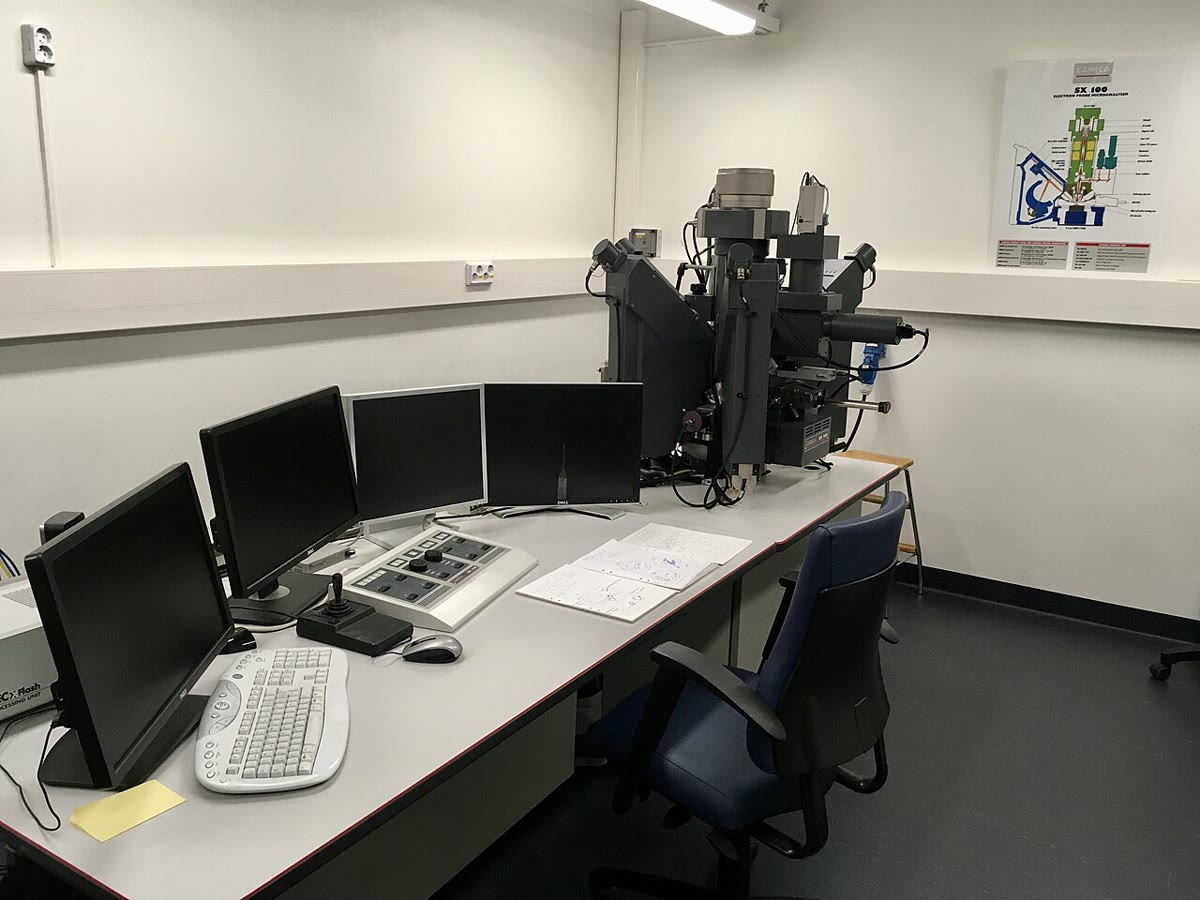
\includegraphics[width=\linewidth]{images/book4/b2-31-microprobe.jpg}
\par\smallskip{\scriptsize एक \omterm{def:b2:field-lab-methods-2:epma}{इलेक्ट्रॉन माइक्रोप्रोब}: इलेक्ट्रॉन स्तंभ, उसके चारों ओर उसके स्पेक्ट्रोमीटर,
और संचालक की मेज़। फ़ोटो: Kallerna, CC BY-SA 4.0 (Wikimedia Commons)।}
\end{minipage}
\end{inthelab}
% ledger: sercE:epma-spot, sercE:coating, photo:b2-31-microprobe

\section{समस्थानिक विश्लेषण}\label{sec:b2:field-lab-methods-2:isotopes}

\omterm{def:b2:isotope-geochemistry:tracer}{रेडियोजनित समस्थानिक अनुरेखक} और आयु (\cref{ch:b2:isotope-geochemistry}) उन अनुपातों पर टिके हैं जो
0.01--\qty{0.001}{\percent} तक मापे जाते हैं, उन तत्त्वों पर जिन्हें चट्टान से विलयन
और आयन-विनिमय क्रोमैटोग्राफ़ी द्वारा किसी स्वच्छ प्रयोगशाला में अलग किया गया हो, जिसकी वायु छनी हुई हो (प्रायः श्रेणी 100 से
1000), ताकि धूल विश्लेषित की जाने वाली अल्प मात्राओं में कुछ न जोड़े।
% ledger: sercT:tims

\begin{definition}[तापीय आयनन द्रव्यमान स्पेक्ट्रममिति, बहु-संग्राहक ICP-MS, द्रव्यमान पूर्वाग्रह]\label{def:b2:field-lab-methods-2:tims}
\emph{तापीय आयनन द्रव्यमान स्पेक्ट्रममिति}\index{तापीय आयनन द्रव्यमान स्पेक्ट्रममिति} (TIMS) में, एक
शुद्ध किया गया तत्त्व धातु के एक पतले फीते पर रखा जाता है और निर्वात में उसे गर्म करके आयनित किया जाता है; आयन
\qty{10}{kV} तक के विभव से त्वरित किए जाते हैं, एक चुंबकीय सेक्टर में द्रव्यमान के अनुसार अलग किए जाते हैं
और संगृहीत होते हैं। \emph{बहु-संग्राहक ICP-MS}\index{बहु-संग्राहक ICP-MS} में आयन एक
प्रेरणिक युग्मित प्लाज़्मा से आते हैं, जो उन तत्त्वों को आयनित करता है जिन्हें तापीय रूप से आयनित करना कठिन है, और कई
संग्राहक भिन्न द्रव्यमानों के पुंजों को एक ही समय मापते हैं। किसी मापन की \emph{द्रव्यमान
पूर्वाग्रह}\index{द्रव्यमान पूर्वाग्रह} मापे गए समस्थानिक अनुपात का नमूने के सच्चे अनुपात से वह विचलन है
जो उपकरण के कारण होता है, जो एक द्रव्यमान को दूसरे की अपेक्षा अधिक सरलता से
संचारित या आयनित करता है।
\end{definition}
% ledger: sercT:tims, sercM:mcicpms

दोनों उपकरण यह परिशुद्धता प्राप्त करते हैं। TIMS सामान्यतः
\qty{1}{\percent} से कम परमाणुओं को आयनित करता है, और उसका \omterm{def:b2:field-lab-methods-2:tims}{द्रव्यमान पूर्वाग्रह} किसी रन के दौरान लगातार बदलता रहता है। पूर्वाग्रह का संशोधन उन दो समस्थानिकों का अनुपात स्थिर मानकर किया जाता है जिन्हें कोई
क्षय नहीं बदलता, जिसके लिए कम से कम तीन समस्थानिकों वाला तत्त्व चाहिए, जिनमें से दो स्थायी हों और
रेडियोजनित न हों। स्ट्रॉन्शियम के लिए $^{86}\mathrm{Sr}/^{88}\mathrm{Sr}$ को 0.1194 पर स्थिर रखा जाता है, और संशोधन का
एक सामान्य रूप चरघातांकी नियम है।
% ledger: sercT:tims, sercM:mcicpms, cheong14:mass-bias, ciaaw:sr-isotopes

\begin{proposition}[द्रव्यमान पूर्वाग्रह का चरघातांकी नियम]\label{prop:b2:field-lab-methods-2:bias}
मान लीजिए द्रव्यमानों $m_i$ और $m_j$ वाले दो समस्थानिकों का हर मापा गया अनुपात सच्चे
अनुपात से $R_{ij}^{\mathrm{true}} = R_{ij}^{\mathrm{meas}}\,(m_i/m_j)^{\beta}$ द्वारा संबंधित है, जहाँ पूरे रन के लिए एक ही घातांक
$\beta$ है। तब किसी संदर्भ युग्म का मापा गया अनुपात $r$, जिसका सच्चा मान
$r_0$ ज्ञात है, देता है
\begin{equation}
\beta = \frac{\ln(r_0/r)}{\ln(m_k/m_l)}
\label{eq:b2:field-lab-methods-2:beta}
\end{equation}
संदर्भ युग्म $k/l$ के लिए, और हर अन्य अनुपात उसी $\beta$ से संशोधित किया जाता है।
\end{proposition}

\begin{proof}
संदर्भ युग्म पर लागू करने पर नियम कहता है $r_0 = r\,(m_k/m_l)^\beta$; लघुगणक लेने पर,
$\ln(r_0/r) = \beta\ln(m_k/m_l)$, जो \eqref{eq:b2:field-lab-methods-2:beta} है। परिकल्पना से घातांक
रन के सभी अनुपातों में उभयनिष्ठ है, इसलिए वह उनमें से हर एक को संशोधित करता है।
\end{proof}

स्ट्रॉन्शियम के लिए संदर्भ युग्म $^{86}\mathrm{Sr}/^{88}\mathrm{Sr}$ है, $r_0 = 0.1194$ के साथ, और
संशोधित $^{87}\mathrm{Sr}/^{86}\mathrm{Sr}$ मापा गया अनुपात गुणा
$(m_{87}/m_{86})^\beta$ है। CIAAW की प्रचुरताएँ, स्ट्रॉन्शियम-86 का \qty{9.86}{\percent} और
स्ट्रॉन्शियम-88 का \qty{82.58}{\percent}, वही मान देती हैं। हर सत्र एक \omterm{def:b2:isotope-geochemistry:standards}{समस्थानिक
संदर्भ मानक} भी चलाता है: एक प्रयोगशाला ने संदर्भ पदार्थ NBS~987 पर सात रनों में $^{87}\mathrm{Sr}/^{86}\mathrm{Sr} = 0.710252 \pm
0.000007$ मापा।
% ledger: cheong14:mass-bias, ciaaw:sr-isotopes

केवल अनुपात सांद्रता नहीं देते। उसके लिए, एक \emph{स्पाइक} की ज्ञात मात्रा, जो किसी एक समस्थानिक में
कृत्रिम रूप से समृद्ध किए गए तत्त्व का विलयन है, रसायन-प्रक्रिया से पहले विलयित नमूने के साथ मिलाई जाती है,
और अनुपात मिश्रण में मापा जाता है। TIMS प्रयोगशालाएँ इसका उपयोग सांद्रताओं
और जनक-से-संतति अनुपातों, दोनों के लिए करती हैं।
% ledger: sercT:tims

\begin{proposition}[समस्थानिक तनुकरण]\label{prop:b2:field-lab-methods-2:id}
मान लीजिए किसी नमूने में $N_x$ मोल एक संदर्भ समस्थानिक $b$ के हैं और किसी स्पाइक में उसके $N_s$ मोल, और मान लीजिए
$R_x$, $R_s$ और $R_m$ नमूने, स्पाइक और मिश्रण में एक दूसरे समस्थानिक $a$ के $b$ से
अनुपात हैं। तब
\begin{equation}
N_x = N_s\,\frac{R_s - R_m}{R_m - R_x} .
\label{eq:b2:field-lab-methods-2:id}
\end{equation}
सापेक्ष त्रुटि $\varepsilon$ के $R_m$ पर होने से $N_x$ को सापेक्ष त्रुटि $\mathcal{M}\varepsilon$ मिलती है,
जहाँ त्रुटि-आवर्धन है
\begin{equation}
\mathcal{M} = \frac{R_m\,(R_s - R_x)}{(R_s - R_m)(R_m - R_x)} ,
\label{eq:b2:field-lab-methods-2:mag}
\end{equation}
जो $R_m = \sqrt{R_s R_x}$ होने पर सबसे छोटा होता है।
\end{proposition}
\index{समस्थानिक तनुकरण}

\begin{proof}
समस्थानिक $a$ मिश्रण में संरक्षित रहता है: $R_m(N_x + N_s) = R_x N_x + R_s N_s$, अतः $N_x(R_m - R_x) =
N_s(R_s - R_m)$, जो \eqref{eq:b2:field-lab-methods-2:id} है। इसका लघुगणकीय अवकलज
$\mathrm{d}\ln N_x/\mathrm{d}\ln R_m = R_m\,[-1/(R_s - R_m) - 1/(R_m - R_x)] = -\mathcal{M}$ है, जहाँ
$\mathcal{M}$ \eqref{eq:b2:field-lab-methods-2:mag} जैसा है। धनात्मक नियतांक $R_s - R_x$ को छोड़कर,
$1/\mathcal{M} = (R_s - R_m)(R_m - R_x)/R_m = R_s + R_x - R_m - R_sR_x/R_m$, जिसका अवकलज
$-1 + R_sR_x/R_m^2$ बिंदु $R_m = \sqrt{R_sR_x}$ पर शून्य होता है, जो $1/\mathcal{M}$ का अधिकतम है।
\end{proof}

\omterm{prop:b2:field-lab-methods-2:id}{समस्थानिक तनुकरण} को न अंशांकन रेखा चाहिए, न रसायन-प्रक्रिया में तत्त्व की
पूर्ण पुनर्प्राप्ति: स्पाइक और नमूना एक बार मिल जाएँ, तो हानियाँ दोनों को समान रूप से प्रभावित करती हैं। उदाहरण के लिए, एक प्रकाशित स्ट्रॉन्शियम
स्पाइक में \qty{99.65}{\percent} स्ट्रॉन्शियम-84 है, जिसमें
$^{84}\mathrm{Sr}/^{88}\mathrm{Sr} = 561.4$ और $^{86}\mathrm{Sr}/^{88}\mathrm{Sr} = 0.7661$ हैं, और
विलयन के प्रति ग्राम \qty{15.271}{\micro\gram} स्ट्रॉन्शियम। इसका 86/88 अनुपात दिखाता है कि
स्पाइक मिले मिश्रण के \omterm{def:b2:field-lab-methods-2:tims}{द्रव्यमान पूर्वाग्रह} का संशोधन $^{86}\mathrm{Sr}/^{88}\mathrm{Sr}$ को उसके
प्राकृतिक मान पर स्थिर करके क्यों नहीं किया जा सकता: स्पाइक ने वह अनुपात खिसका दिया है।
% ledger: cheong14:spike, cheong14:mass-bias

\section{वार्डन इनलायर पर एक मानचित्रण अभियान}\label{sec:b2:field-lab-methods-2:campaign}

वार्डन अपनति के क्रोड में, अपरदन ने बलुआ पत्थर के आवरण को काटकर
आधार-शैल को अनावृत कर दिया है: ग्रेनाइट द्वारा अंतर्वेधित शिस्ट। प्रयोगशाला को सामग्री देने वाला अभियान
क्षेत्र में आरंभ होता है। इनलायर के आर-पार पश्चिम से पूर्व की ओर दो अनुप्रस्थ मार्ग चले जाते हैं, हर
\qty{100}{m} पर एक स्टेशन के साथ; हर स्टेशन पर इकाई दर्ज की जाती है, और जहाँ चट्टान
अपक्षयित नहीं है वहाँ ताज़े नमूने लिए जाते हैं, स्टेशन के अंक से क्रमांकित, और जहाँ विन्यास मापे जाने हों वहाँ अभिमुखित। चित्र
दिखाता है कि स्टेशनों पर क्या मिलता है: 30 में से दस ग्रेनाइट पर हैं, दस बलुआ पत्थर के आवरण पर, एक
शिस्ट पर, एक चूना-पत्थर पर और आठ घाटी-तल के जलोढ़ पर, जहाँ कोई चट्टान अनावृत
नहीं होती।

\begin{omfigure}
\centering
\begin{tikzpicture}
\begin{axis}[axis equal image, xmin=2.4, xmax=4.6, ymin=3.1, ymax=5.0, width=0.66\linewidth,
  tick label style={font=\scriptsize}, xlabel={पूर्व (km)}, ylabel={उत्तर (km)},
  label style={font=\small}]
% units: figdata/shared/region.py (read only); stations: figdata/bachelor-2/labmethods.py part stations
\addplot[lith schist, draw=black, line width=0.3pt, even odd rule] table {figdata/out/shared-region-unit-schist.dat};
\addplot[lith granite, draw=black, line width=0.3pt, even odd rule] table {figdata/out/shared-region-unit-granite.dat};
\addplot[om lith={icsTriassic!35}{om sand}, draw=black, line width=0.3pt, even odd rule] table {figdata/out/shared-region-unit-sandstone.dat};
\addplot[om lith={icsJurassic!40}{om limestone}, draw=black, line width=0.3pt, even odd rule] table {figdata/out/shared-region-unit-limestone.dat};
\addplot[om lith={icsJurassic!15}{om shale}, draw=black, line width=0.3pt, even odd rule] table {figdata/out/shared-region-unit-shale.dat};
\addplot[lith alluvium, draw=black, line width=0.3pt, even odd rule] table {figdata/out/shared-region-unit-alluvium.dat};
\addplot[river] table {figdata/out/shared-region-river.dat};
\addplot[only marks, mark=*, mark size=1.6pt, mark options={fill=white, draw=black}]
  table[x=x_km, y=y_km] {figdata/out/bachelor-2-labmethods-stations.dat};
\addplot[only marks, mark=*, mark size=1.6pt, mark options={fill=omThm, draw=black},
  x filter/.expression={\thisrow{unit}==2 ? x : nan}]
  table[x=x_km, y=y_km] {figdata/out/bachelor-2-labmethods-stations.dat};
\node[font=\scriptsize, fill=white, inner sep=1pt, anchor=east] at (axis cs:2.76,3.7) {1};
\node[font=\scriptsize, fill=white, inner sep=1pt, anchor=west] at (axis cs:4.24,3.7) {15};
\node[font=\scriptsize, fill=white, inner sep=1pt, anchor=east] at (axis cs:2.76,4.4) {16};
\node[font=\scriptsize, fill=white, inner sep=1pt, anchor=west] at (axis cs:4.24,4.4) {30};
\draw[black, line width=0.5pt] (axis cs:3.5,4.44) -- (axis cs:3.5,4.62);
\node[font=\scriptsize, fill=white, inner sep=1pt, anchor=south] at (axis cs:3.5,4.62) {स्टेशन 23};
\pic at (axis cs:4.45,4.75) {northarrow};
\end{axis}
\end{tikzpicture}
\par\smallskip{\small वार्डन पहाड़ियों का आधार-शैल इनलायर, दो पश्चिम--पूर्व
अनुप्रस्थ मार्गों के 30 स्टेशनों के साथ, जो \qty{100}{m} दूर हैं। लाल बिंदु: ग्रेनाइट पर स्टेशन। क्रॉस वाला गुलाबी: ग्रेनाइट; धूसर: शिस्ट; बैंगनी: ट्राइऐसिक
बलुआ पत्थर; नीला: जुरासिक चूना-पत्थर; हल्का नीला: जुरासिक शेल; क्रीम: नदी का जलोढ़, जो
पूर्व की ओर बहती है।
सप्ताहांत समस्या का ग्रेनाइट नमूना स्टेशन 23 से आता है।}
\end{omfigure}

\begin{inthefield}[प्रयोगशाला के लिए नमूना-संग्रह]
\centering
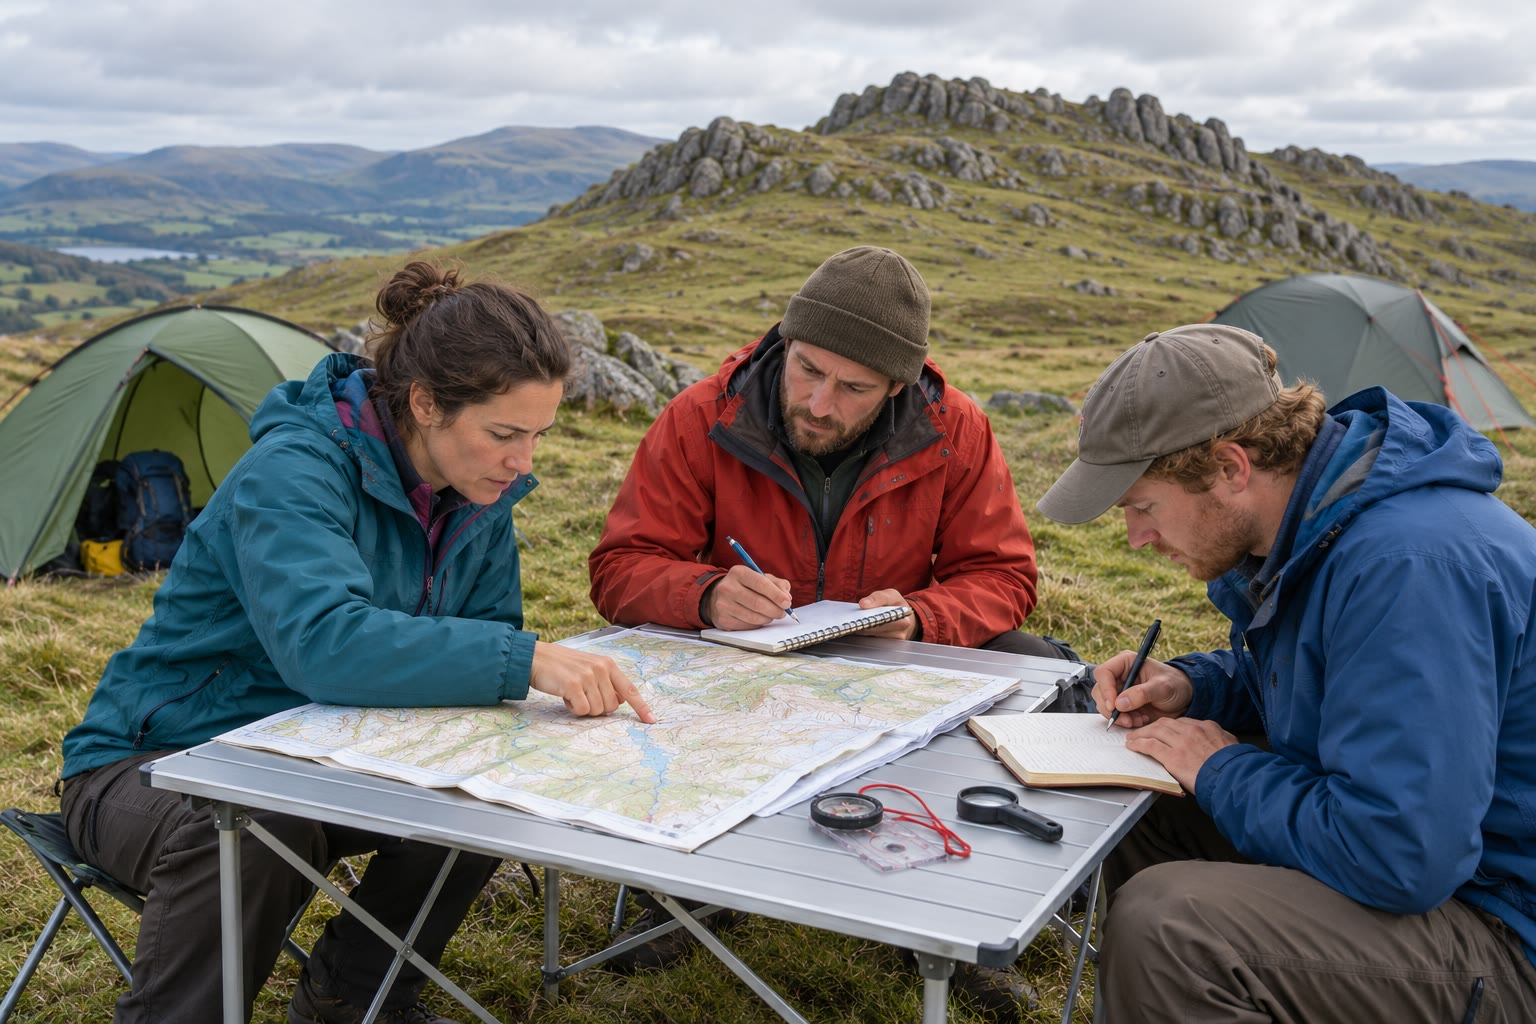
\includegraphics[width=0.56\linewidth]{images/book4/ai/b2-field-camp.jpg}
\par\smallskip{\small एक क्षेत्र-दल अगले दिन के अनुप्रस्थ मार्गों की योजना बनाता है (AI से बनाया गया चित्रण)।}
\par\medskip\raggedright
शाम को दल स्टेशनों को मानचित्र पर उतारता है, जाँचता है कि नोटबुकों का हर नमूना-अंक
किसी थैले से मेल खाता है, और तय करता है कि कौन से नमूने किस प्रयोगशाला में जाएँगे। हर इकाई का एक नमूना
पतली-काट प्रयोगशाला में जाता है; सबसे ताज़े ग्रेनाइट और शिस्ट
कुचलने और संपूर्ण-शैल विश्लेषण के लिए जाते हैं; ग्रेनाइट के कुछ नमूने समस्थानिकों के लिए अलग रखे जाते हैं।
स्टेशन-अंक हर नमूने के साथ हर चरण से गुज़रता है, थैले से पतली काट, चूर्ण, गुटिका और
आँकड़ा-तालिका की पंक्ति तक, ताकि किसी भी विचित्र परिणाम का पता उसके
अनावरण तक लगाया जा सके।
\end{inthefield}

\section{किसी संख्या की गुणवत्ता}\label{sec:b2:field-lab-methods-2:quality}

शृंखला का हर चरण अपनी त्रुटि जोड़ता है, और इस अध्याय की विधियाँ वे दोनों प्रकार दिखाती हैं जिनमें
रसायन की पुस्तकें भेद करती हैं। \omterm{def:b2:field-lab-methods-2:modal}{बिंदु-गणना} और समस्थानिक अनुपातों में अधिकतर यादृच्छिक त्रुटियाँ होती हैं, जो
गणनाएँ बढ़ने पर $1/\sqrt n$ की तरह सिकुड़ती हैं; अंशांकन में व्यवस्थित त्रुटियाँ होती हैं, जिन्हें पुनरावृत्ति
कम नहीं करती और जिन्हें केवल कोई संदर्भ पदार्थ प्रकट करता है। सिलिका विश्लेषणों का चित्र
दोनों दिखाता है: पट्टियाँ विधि की परिशुद्धता हैं, और जो बिंदु शून्य से अपनी पट्टी को
विश्लेषणों की संख्या के वर्गमूल से भाग देने पर मिली राशि के कई गुना से चूकता है, वह एक पूर्वाग्रह है। दो
विधियों से मापा गया वही तत्त्व, XRF से और \omterm{prop:b2:field-lab-methods-2:id}{समस्थानिक तनुकरण} से स्ट्रॉन्शियम, एक और जाँच है, क्योंकि दोनों का कोई
अंशांकन साझा नहीं है। परिणाम उनकी अनिश्चितता के साथ, उसी तक पूर्णांकित करके, और साथ चलाए गए संदर्भ
पदार्थों के साथ बताए जाते हैं; उनके बिना कोई संख्या किसी अन्य संख्या से तुलनीय नहीं होती।

\section*{अभ्यास}\label{sec:b2:field-lab-methods-2:exercises}

अभ्यासों के लिए आँकड़े, जब तक अन्यथा न कहा जाए: परमाणु द्रव्यमान H 1.008, O 15.999, Mg 24.305, Al
26.982, Si 28.085, K 39.098, Sr 87.62; समस्थानिक द्रव्यमान $^{86}\mathrm{Sr}$ 85.909261,
$^{87}\mathrm{Sr}$ 86.908878, $^{88}\mathrm{Sr}$ 87.905612; प्राकृतिक स्ट्रॉन्शियम
$^{84}\mathrm{Sr}/^{86}\mathrm{Sr} = 0.05680$, \qty{9.86}{\percent} $^{86}\mathrm{Sr}$; पाठ का
स्पाइक, $^{84}\mathrm{Sr}/^{86}\mathrm{Sr} = 732.8$, \qty{0.13599}{\percent} $^{86}\mathrm{Sr}$,
परमाणु भार 83.9242, \qty{15.271}{\micro\gram\per\gram}। जब तक अन्यथा न कहा जाए,
तीन सार्थक अंकों तक पूर्णांकित कीजिए।
% ledger: ciaaw:H, ciaaw:O, ciaaw:Mg, ciaaw:Al, ciaaw:Si, ciaaw:K, ciaaw:sr-isotopes, cheong14:spike

\begin{exercise}[$\star$]\label{exo:b2:field-lab-methods-2:1}
(क) बनावट या क्रिस्टल का नाम बताइए: (i) एक डोलेराइट जिसमें प्लैजियोक्लेज़ की पट्टिकाएँ बड़े ऑगाइट
क्रिस्टलों में पूरी तरह घिरी हैं; (ii) समान आकार के कैल्साइट कणों वाला एक संगमरमर जिनकी सीधी सीमाएँ तीन-तीन करके
मिलती हैं; (iii) किसी अभ्रक शिस्ट में क्वार्ट्ज़ के अंतर्वेशों से भरा \qty{5}{mm} लंबा एक स्टॉरोलाइट क्रिस्टल;
(iv) प्लैजियोक्लेज़ और पाइरॉक्सीन के सतत घेरे से घिरा एक गार्नेट। (ख) तीन कण-सीमाएँ
\ang{104}, \ang{128} और \ang{128} पर मिलती हैं। \ang{104} कोण के सम्मुख सीमा के तनाव का
अन्य सीमाओं के तनाव से अनुपात ज्ञात कीजिए।
\end{exercise}

\begin{exercise}[$\star$]\label{exo:b2:field-lab-methods-2:2}
एक स्थूल-कणिक चट्टान में \qty{25}{\percent} क्वार्ट्ज़, 15 क्षार-फ़ेल्डस्पार, 40 प्लैजियोक्लेज़, 12
बायोटाइट और 8 हॉर्नब्लेंड है। (क) Q, A और P पुनः परिकलित कीजिए। (ख) P/(A+P) ज्ञात कीजिए और चट्टान का नाम बताइए। (ग) उसका
रंग-सूचकांक ज्ञात कीजिए और उसे वर्गीकृत कीजिए।
\end{exercise}

\begin{exercise}[$\star$]\label{exo:b2:field-lab-methods-2:3}
800 बिंदुओं की एक गणना किसी खनिज को \qty{12}{\percent} पर पाती है। (क) इस अनुपात का मानक विचलन,
और उसका सापेक्ष मान, ज्ञात कीजिए। (ख) 3200 बिंदुओं के साथ वह क्या होता?
\end{exercise}

\begin{exercise}[$\star$]\label{exo:b2:field-lab-methods-2:4}
\qty{0.8000}{g} का एक चूर्ण प्रज्वलन के बाद \qty{0.7712}{g} तौलता है, और अवशेष को
\qty{8.0000}{g} गालक के साथ संगलित किया जाता है। (क) \omterm{def:b2:field-lab-methods-2:xrf}{प्रज्वलन-हानि} ज्ञात कीजिए। (ख) गुटिका में नमूने का
द्रव्यमान-अंश ज्ञात कीजिए। (ग) काँच में \qty{5.20}{\percent} \ce{SiO2} है। प्रज्वलित चूर्ण की
और मूल चूर्ण की सिलिका ज्ञात कीजिए।
\end{exercise}

\begin{exercise}[$\star\star$]\label{exo:b2:field-lab-methods-2:5}
(क) किसी चट्टान का \qty{2}{\percent} बनाने वाले किसी सहायक खनिज को
\qty{10}{\percent} की सापेक्ष मानक त्रुटि के साथ मापने के लिए कितने बिंदु चाहिए? (ख) और \qty{30}{\percent} बनाने वाले किसी खनिज के लिए,
उसी सापेक्ष त्रुटि के साथ? (ग) किसी दुर्लभ खनिज द्वारा माँगे जाने वाले श्रम पर टिप्पणी कीजिए।
\end{exercise}

\begin{exercise}[$\star\star$]\label{exo:b2:field-lab-methods-2:6}
चित्र के USGS परिणामों में, रायोलाइट RGM-1 ने 20 विश्लेषणों में \ce{SiO2} $= 72.89$ दिया, मानक
विचलन 0.19 के साथ (अनुशंसित 73.45), और बेसाल्ट BCR-2 ने 54.17, 0.13 के साथ, 20
विश्लेषणों में (अनुशंसित 54.1)। (क) प्रतिशत में हर एक की पुनर्प्राप्ति ज्ञात कीजिए। (ख) हर माध्य का मानक
विचलन ज्ञात कीजिए, और अनुशंसित मान से हर अंतर को उसकी इकाइयों में व्यक्त कीजिए।
(ग) कौन सा परिणाम पूर्वाग्रह दिखाता है? क्या RGM-1 के लिए विधि कम परिशुद्ध है?
\end{exercise}

\begin{exercise}[$\star\star$]\label{exo:b2:field-lab-methods-2:7}
एक शुद्ध फ़्लोगोपाइट, $\mathrm{KMg_3AlSi_3O_{10}(OH)_2}$, के एक माइक्रोप्रोब विश्लेषण की जाँच करनी है।
(क) सूत्र का मोलर द्रव्यमान और उसमें निहित \ce{H2O} का द्रव्यमान-अंश ज्ञात कीजिए। (ख)
\ce{K2O}, \ce{MgO}, \ce{Al2O3} और \ce{SiO2} के द्रव्यमान-अंश, और वह योग ज्ञात कीजिए जो कोई यथार्थ विश्लेषण
देगा। (ग) किसी अभ्रक के लिए लगभग \qty{96}{\percent} का योग खराब विश्लेषण क्यों नहीं है?
\end{exercise}

\begin{exercise}[$\star\star$]\label{exo:b2:field-lab-methods-2:8}
किसी स्ट्रॉन्शियम मानक पर एक TIMS रन $^{86}\mathrm{Sr}/^{88}\mathrm{Sr} = 0.11905$ और
$^{87}\mathrm{Sr}/^{86}\mathrm{Sr} = 0.71062$ देता है। (क) चरघातांकी नियम का घातांक $\beta$ ज्ञात कीजिए।
(ख) $^{87}\mathrm{Sr}/^{86}\mathrm{Sr}$ अनुपात को पाँच दशमलव स्थानों तक संशोधित कीजिए। (ग) रन में हल्के
या भारी समस्थानिक में से किसे वरीयता मिली?
\end{exercise}

\begin{exercise}[$\star\star$]\label{exo:b2:field-lab-methods-2:9}
अपने \omterm{prop:b2:field-lab-methods-2:id}{समस्थानिक तनुकरण} की जाँच के लिए, एक प्रयोगशाला संदर्भ बेसाल्ट BHVO-2 के \qty{0.0500}{g} में
पाठ के स्पाइक का \qty{0.1000}{g} मिलाती है, और मिश्रण में $^{84}\mathrm{Sr}/^{86}\mathrm{Sr} =
0.874$ मापती है। (क) स्पाइक के अंश में $^{86}\mathrm{Sr}$ के मोल ज्ञात कीजिए। (ख) नमूने में
$^{86}\mathrm{Sr}$ के मोल, और ppm में उसकी स्ट्रॉन्शियम सांद्रता ज्ञात कीजिए। (ग) अनुशंसित
\qty{394.1}{ppm} से तुलना कीजिए।
\end{exercise}

\begin{exercise}[$\star\star\star$]\label{exo:b2:field-lab-methods-2:10}
पाठ के स्ट्रॉन्शियम स्पाइक के लिए ($R_s = 732.8$, $R_x = 0.05680$): (क) मिश्रण का वह अनुपात ज्ञात कीजिए
जो त्रुटि-आवर्धन को न्यूनतम करता है, और वहाँ उसका मान; (ख) $\mathcal M$ का मान
$R_m = 0.1$, 0.5, 1.664 और 100 पर निकालिए; (ग) समझाइए कि किसी भी अंत्य-सदस्य के निकट के मिश्रण से क्यों
बचना चाहिए, और व्यवहार में विश्लेषक के पास कितनी स्वतंत्रता है।
\end{exercise}

\begin{exercise}[$\star\star\star$]\label{exo:b2:field-lab-methods-2:11}
एक ग्रेनाइट-गणना 400 फ़ेल्डस्पार बिंदु पाती है, जिनमें से \qty{62}{\percent} प्लैजियोक्लेज़ हैं। (क) फ़ेल्डस्पार बिंदुओं में
प्लैजियोक्लेज़ को द्विपद गणना मानकर
P/(A+P) का मानक विचलन ज्ञात कीजिए। (ख) परिणाम ग्रैनोडायोराइट सीमा से कितने मानक विचलन दूर है? (ग) कितने
फ़ेल्डस्पार बिंदु उसे सीमा से दो मानक विचलन दूर रखेंगे?
\end{exercise}

\begin{exercise}[$\star\star\star$]\label{exo:b2:field-lab-methods-2:12}
कोई खनिज किसी चट्टान का अंश $p$ घेरता है। (क) दिखाइए कि इसकी प्रायिकता कि $n$ स्वतंत्र
बिंदु सभी उससे चूक जाएँ, $(1-p)^n$ है। (ख) कितने बिंदु कम से कम \qty{95}{\percent} की यह प्रायिकता देते हैं कि
चट्टान का \qty{1}{\percent} बनाने वाला खनिज कम से कम एक बार मिल जाए? (ग) यही \qty{0.05}{\percent} पर ज़िरकॉन के लिए
कीजिए, और निष्कर्ष निकालिए कि किसी सहायक खनिज को कैसे खोजा जाना चाहिए।
\end{exercise}

\section*{सप्ताहांत समस्या}

\begin{problem}[{सप्ताहांत समस्या --- अनावरण से विश्लेषण तक}]\label{pb:b2:field-lab-methods-2:1}
% invented sample; data: ledger rows below; values: calc/ch31.py
वार्डन ग्रेनाइट का नमूना VH-23 अभियान के स्टेशन 23 पर लिया गया। एक पतली काट की
1200 बिंदुओं के नियमित ग्रिड पर \omterm{def:b2:field-lab-methods-2:modal}{बिंदु-गणना} की गई: क्वार्ट्ज़ 372, क्षार-फ़ेल्डस्पार 348, प्लैजियोक्लेज़ 324,
बायोटाइट 108, मस्कोवाइट 36, अपारदर्शी ऑक्साइड 12। \qty{0.8000}{g} का एक चूर्ण प्रज्वलन के बाद \qty{0.7949}{g} तौला गया
(प्रज्वलन \qty{925}{\celsius} पर) और \qty{8.0000}{g} गालक के साथ संगलित किया गया। तीन
संदर्भ पदार्थों की गुटिकाओं ने ये \ce{SiO2} तीव्रताएँ दीं (हज़ार गणनाएँ प्रति सेकंड, kcps): BCR-2,
अनुशंसित \qty{54.1}{\percent}, 21.66; AGV-2, 59.3, 23.70; RGM-1, 73.45, 29.37; ग्रेनाइट की गुटिका ने
28.63 दिया। ग्रेनाइट के अन्य ऑक्साइडों का योग \qty{27.15}{\percent} है। समस्थानिकों के लिए,
\qty{0.1000}{g} चूर्ण को विलयित करके पाठ के स्पाइक के \qty{0.2500}{g} के साथ मिलाया गया;
नमूने में अभ्यासों की प्राकृतिक स्ट्रॉन्शियम प्रचुरताएँ मानी जाती हैं। अभ्यासों के
आँकड़ों का उपयोग कीजिए।

\noindent\textbf{भाग I --- मोड।}
\begin{enumerate}
  \item हर खनिज का मोडल अनुपात ज्ञात कीजिए।
  \item क्वार्ट्ज़ अनुपात का मानक विचलन, और मस्कोवाइट अनुपात का सापेक्ष मानक विचलन
        ज्ञात कीजिए।
  \item $M$ और रंग-सूचकांक $M'$ ज्ञात कीजिए, और चट्टान को वर्गीकृत कीजिए।
  \item Q, A और P को 100 के योग पर पुनः परिकलित कीजिए।
  \item P/(A+P) ज्ञात कीजिए और \omterm{def:b2:magmatic-series:qapf}{QAPF आरेख} पर चट्टान का नाम बताइए।
  \item 672 फ़ेल्डस्पार बिंदुओं पर P/(A+P) के द्विपद मानक विचलन के साथ, क्या यह नाम
        सुरक्षित है?
  \item कितने बिंदु क्वार्ट्ज़ अनुपात के मानक विचलन को एक
        प्रतिशत-अंक तक ले आएँगे?
\end{enumerate}

\noindent\textbf{भाग II --- एक्स-किरण प्रतिदीप्ति से सिलिका।}
\begin{enumerate}[resume]
  \item \omterm{def:b2:field-lab-methods-2:xrf}{प्रज्वलन-हानि} ज्ञात कीजिए।
  \item गुटिका में नमूने का द्रव्यमान-अंश ज्ञात कीजिए, और काँच की सिलिका, यदि
        प्रज्वलित चूर्ण में \qty{72}{\percent} हो।
  \item तीन संदर्भ पदार्थों से होकर न्यूनतम-वर्ग रेखा $c = aI + b$ समंजित कीजिए; $a$ को
        चार दशमलव स्थानों तक और $b$ को दो तक दीजिए।
  \item ग्रेनाइट का \ce{SiO2} दो दशमलव स्थानों तक ज्ञात कीजिए।
  \item तीन संदर्भ पदार्थों के अवशिष्ट ज्ञात कीजिए। क्या रेखा पर्याप्त है?
  \item ऑक्साइडों और \omterm{def:b2:field-lab-methods-2:xrf}{प्रज्वलन-हानि} को जोड़िए। क्या USGS प्रक्रिया यह विश्लेषण दोहराएगी?
  \item वाष्पशीलों के बिना सिलिका को 100 के योग पर पुनः परिकलित कीजिए।
\end{enumerate}

\noindent\textbf{भाग III --- द्रव्यमान पूर्वाग्रह।}
\begin{enumerate}[resume]
  \item CIAAW की प्रचुरताओं से प्राकृतिक $^{86}\mathrm{Sr}/^{88}\mathrm{Sr}$ ज्ञात कीजिए और उसकी तुलना
        प्रसामान्यीकरण में प्रयुक्त मान से कीजिए।
  \item स्पाइक-रहित एक अंश $^{86}\mathrm{Sr}/^{88}\mathrm{Sr} = 0.11853$ देता है। $\beta$ को
        चार दशमलव स्थानों तक ज्ञात कीजिए।
  \item वह $^{87}\mathrm{Sr}/^{86}\mathrm{Sr} = 0.71655$ देता है। इसे पाँच दशमलव स्थानों तक संशोधित कीजिए।
  \item प्रतिशत में प्रति द्रव्यमान-इकाई पूर्वाग्रह ज्ञात कीजिए।
  \item यह संशोधन भाग IV के स्पाइक मिले मिश्रण पर क्यों नहीं किया जा सकता?
\end{enumerate}

\noindent\textbf{भाग IV --- समस्थानिक तनुकरण।}
\begin{enumerate}[resume]
  \item जाँचिए कि स्पाइक में \qty{99.65}{\percent} स्ट्रॉन्शियम-84 और \qty{0.13599}{\percent}
        स्ट्रॉन्शियम-86 है।
  \item स्पाइक के अंश में स्ट्रॉन्शियम के और $^{86}\mathrm{Sr}$ के मोल, चार सार्थक अंकों तक,
        ज्ञात कीजिए।
  \item अभ्यासों के मान $R_s = 732.8$ और $R_x = 0.05680$ जाँचिए।
  \item मिश्रण का संशोधित अनुपात $R_m = 1.6812$ है। नमूने के $^{86}\mathrm{Sr}$ के मोल
        ज्ञात कीजिए।
  \item त्रुटि-आवर्धन ज्ञात कीजिए। $R_m$ के \qty{0.01}{\percent} तक और स्पाइक की
        सांद्रता के $\pm\qty{0.031}{\micro\gram\per\gram}$ तक ज्ञात होने पर, परिणाम की सापेक्ष
        अनिश्चितता ज्ञात कीजिए।
  \item वार्डन ग्रेनाइट की स्ट्रॉन्शियम सांद्रता ppm में ज्ञात कीजिए।
\end{enumerate}
\end{problem}
% ledger: bgsI:qapf, bgsI:colour-index, usgsT:procedure, usgsT:sio2-table, ciaaw:sr-isotopes, cheong14:spike, cheong14:mass-bias
